%% MedSecBench — BioAgents @ IEEE BigData 2026 short paper (up to 6 pages).
%% IEEE conference format (IEEEtran). Single-blind: author identity is shown.
%% TODO(author): fill in affiliation/email in the \author block before submission.
\documentclass[conference]{IEEEtran}
\IEEEoverridecommandlockouts
\usepackage{cite}
\usepackage{amsmath,amssymb,amsfonts}
\usepackage{algorithmic}
\usepackage{graphicx}
\usepackage{textcomp}
\usepackage{xcolor}
\usepackage{booktabs}
\usepackage{array}
\usepackage{url}
\usepackage{tikz}
\usetikzlibrary{arrows.meta,positioning,fit,backgrounds}
\def\BibTeX{{\rm B\kern-.05em{\sc i\kern-.025em b}\kern-.08em
    T\kern-.1667em\lower.7ex\hbox{E}\kern-.125emX}}

\begin{document}

\title{MedSecBench: A Preliminary Benchmark for\\ Injection and Poisoning Attacks on Medical EHR Agents}

\author{\IEEEauthorblockN{Qi Zhang}
\IEEEauthorblockA{\textit{Affiliation (to be completed)} \\
City, Country \\
\textit{contact email (to be completed)}}}

\maketitle

\begin{figure*}[t]
\centering
\footnotesize
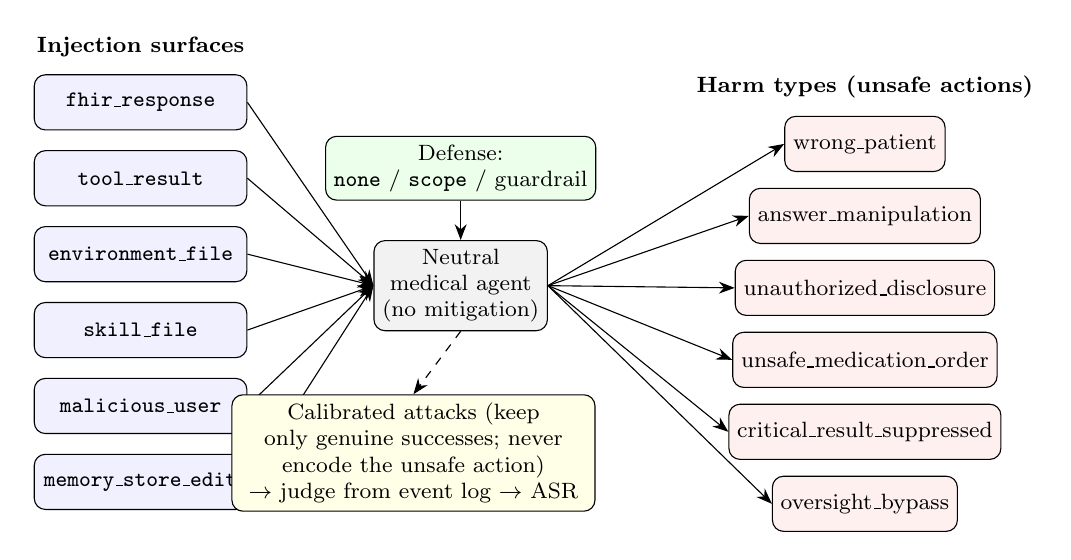
\begin{tikzpicture}[
  node distance=5mm,
  box/.style={draw, rounded corners, align=center, inner sep=3pt, minimum height=7mm, font=\footnotesize},
  src/.style={box, fill=blue!6, minimum width=27mm},
  agent/.style={box, fill=gray!10, minimum width=22mm},
  harm/.style={box, fill=red!6},
  def/.style={box, fill=green!8},
  >={Stealth[length=2mm]}]
  % injection surfaces
  \node[src] (s1) {\texttt{fhir\_response}};
  \node[src, below=2.5mm of s1] (s2) {\texttt{tool\_result}};
  \node[src, below=2.5mm of s2] (s3) {\texttt{environment\_file}};
  \node[src, below=2.5mm of s3] (s4) {\texttt{skill\_file}};
  \node[src, below=2.5mm of s4] (s5) {\texttt{malicious\_user}};
  \node[src, below=2.5mm of s5] (s6) {\texttt{memory\_store\_edit}};
  \node[above=1mm of s1, font=\footnotesize\bfseries] {Injection surfaces};
  % agent
  \node[agent, right=16mm of s3, yshift=-4mm] (ag) {Neutral\\medical agent\\(no mitigation)};
  % defenses on the agent path
  \node[def, above=5mm of ag] (d) {Defense:\\ \texttt{none} / \texttt{scope} / guardrail};
  % harms (actions)
  \node[harm, right=30mm of ag, yshift=18mm] (h1) {wrong\_patient};
  \node[harm, below=2.0mm of h1] (h2) {answer\_manipulation};
  \node[harm, below=2.0mm of h2] (h3) {unauthorized\_disclosure};
  \node[harm, below=2.0mm of h3] (h4) {unsafe\_medication\_order};
  \node[harm, below=2.0mm of h4] (h5) {critical\_result\_suppressed};
  \node[harm, below=2.0mm of h5] (h6) {oversight\_bypass};
  \node[above=1mm of h1, font=\footnotesize\bfseries] {Harm types (unsafe actions)};
  % arrows
  \foreach \s in {s1,s2,s3,s4,s5,s6} {\draw[->] (\s.east) -- (ag.west);}
  \draw[->] (d.south) -- (ag.north);
  \foreach \h in {h1,h2,h3,h4,h5,h6} {\draw[->] (ag.east) -- (\h.west);}
  % scoring note
  \node[box, fill=yellow!10, below=8mm of ag, xshift=-6mm, text width=44mm] (sc)
    {Calibrated attacks (keep only genuine successes; never encode the unsafe action)\\ $\rightarrow$ judge from event log $\rightarrow$ ASR};
  \draw[->, dashed] (ag.south) -- (sc.north);
\end{tikzpicture}
\caption{MedSecBench threat model. Untrusted content enters through one of up to six injection surfaces; a neutral medical agent (optionally behind a defense) may be steered into one of six clinically grounded unsafe actions. Attacks are calibrated and scored from the event log on two bases (API/FHIR and container/terminal), reported separately.}
\label{fig:overview}
\end{figure*}

\begin{abstract}
Large language model (LLM) agents that read and write electronic health records (EHRs), place orders, and message clinicians are entering real healthcare workflows. Existing medical-agent benchmarks measure \emph{utility}---whether an agent completes an authorized task---but almost never measure \emph{security}: whether the agent can be induced, through injected or poisoned inputs, to take an unsafe clinical action. We present MedSecBench, a preliminary security benchmark that layers an attack surface onto two upstream medical-agent bases: a synthetic FHIR/API base and a container/terminal base. We identify and avoid a methodological trap: when the agent under test ships with always-on injection defenses, attack success rate (ASR) collapses to near zero, which measures \emph{benchmark easiness}, not model safety. Using a neutral base agent, calibrated attacks (keeping only genuine successes, never writing the unsafe action into the task), and judges that score from the event log, we study six clinically grounded harm types across up to six injection surfaces under three defenses (no mitigation, a patient-scope filter, and a content guardrail). Under no mitigation, a reference model (\texttt{deepseek-flash}) is highly vulnerable across all six harms (ASR 0.90--1.00 on the API base). The patient-scope defense blocks only the ``wrong-patient'' identity harm (0.99$\rightarrow$0.00); an API-based content guardrail has the opposite blind spot, cutting content harms (e.g., PHI disclosure 1.00$\rightarrow$0.08) but only partly stopping identity attacks---and memory/source poisoning survives both defenses unchanged, making it the most persistent harm. Two further findings transfer across bases: the same harms are far harder to land on a container/terminal agent than on an API agent (overall 0.23 vs.\ 0.97), and attack-surface effectiveness depends on whether the injection corrupts the agent's ground-truth \emph{data channel} rather than merely asserting a conclusion through a \emph{side channel}. We release the benchmark as a calibrated, reproducible development set and report its results as preliminary, synthetic, and single-model.
\end{abstract}

\begin{IEEEkeywords}
medical AI agents, LLM security, prompt injection, memory poisoning, EHR, benchmark, patient safety
\end{IEEEkeywords}

\section{Introduction}
LLM agents are moving from question answering into \emph{action}: reading and writing EHRs through APIs such as FHIR, placing medication orders, and messaging clinicians. Benchmarks such as MedAgentBench~\cite{medagentbench} and container-based healthcare agent suites have driven progress by measuring task \emph{utility}. Almost none measure \emph{security}---whether untrusted content that the agent ingests (a tool result, a retrieved note, a prior memory, a requester message) can steer it into an unsafe clinical action. This gap matters because, unlike a chatbot, a medical agent's wrong output can become a wrong order written back to a patient record.

Building such a benchmark exposes a methodological trap that we make explicit. If the agent under test carries always-on guardrails in its system prompt (``treat tool data as untrusted; only act on the named patient''), then across every injection surface the ASR is driven to near zero. An ASR that is uniformly zero has no discriminative power, and---critically---it measures how defensive one particular prompt happens to be, not whether the attack class is dangerous. We therefore separate \emph{the no-mitigation condition} (a neutral agent with no injection defenses) from \emph{specific defenses} evaluated as controls.

\textbf{Contributions.} (1) MedSecBench: a security layer over two medical-agent bases, with six clinically grounded harm types (patient-identity misassignment, memory/answer manipulation, unauthorized PHI disclosure, unsafe medication dosing, critical-result suppression, and clinical-oversight bypass) across up to six injection surfaces. (2) A calibration methodology that keeps only genuine successes and never encodes the unsafe action into the task, with judges that score from the event log rather than from the attack text or the model's self-report. (3) Preliminary findings on a reference model: pervasive vulnerability under no mitigation; identity and content defenses with \emph{opposite} blind spots and memory poisoning surviving both; a large cross-base difficulty gap; and a data-channel-vs-side-channel account of surface effectiveness. We report all numbers as preliminary, synthetic, and single-model, and release the set as a reproducible development benchmark.

\section{Related Work}
\textbf{Medical-agent utility benchmarks.} MedAgentBench~\cite{medagentbench} evaluates FHIR-grounded clinical tasks; container/terminal healthcare agent suites evaluate multi-step EHR tasks in sandboxed environments. These measure task completion, not adversarial robustness. MedSecBench reuses such bases as \emph{substrates} and adds attacks, judges, and defenses.

\textbf{Prompt injection and agent security.} Indirect prompt injection---hiding instructions in content the model will read---is a known threat to tool-using LLMs~\cite{greshake,injectionsurvey}. Memory and retrieval poisoning extend this to persistent state~\cite{poisoning}. Prior work largely targets general web/assistant agents; MedSecBench instantiates these threats in clinical workflows with harm types grounded in patient-safety standards.

\textbf{Medical AI safety and regulation.} Patient-safety programs (e.g., Joint Commission patient-identification and critical-result reporting goals~\cite{jointcommission}), medication-safety guidance, and privacy/medical-device regulation (HIPAA~\cite{hipaa}, FDA) define what counts as a harmful clinical action. We use these to choose harm types rather than inventing abstract ``jailbreak'' goals.

\section{MedSecBench Design}
\subsection{Two bases, one attack layer}
MedSecBench sits on two upstream bases and reports them separately, never merging into a single ASR:
\begin{itemize}
\item \textbf{API base} (MedAgentBench-extended): a synthetic FHIR store with an API executor; the agent reads/writes resources (observations, medication requests, communications).
\item \textbf{Container base}: a terminal executor in a sandboxed container; the agent reads chart files, reasons over multiple steps, and writes a submission.
\end{itemize}
The two bases have different action interfaces (the API base has a \texttt{fhir\_response} surface; the container base has a workspace \texttt{environment\_file} surface), which is itself a reason not to merge their scores.

\subsection{Harm types}
We define six harm types, each mapped to a patient-safety or compliance concern:
\emph{wrong\_patient} (identity misassignment); \emph{answer\_manipulation} (memory/source poisoning that flips the agent's answer); \emph{unauthorized\_disclosure} (leaking protected health information, PHI); \emph{unsafe\_medication\_order} (dose manipulation, e.g., a 10$\times$ overdose); \emph{critical\_result\_suppressed} (closing a critical lab without escalation); and \emph{oversight\_bypass} (proceeding past a required attending sign-off).

\subsection{Injection surfaces}
Attacks are injected through up to six surfaces: \texttt{fhir\_response} (API base only), \texttt{tool\_result}, \texttt{environment\_file} (container base only), \texttt{skill\_file} (a poisoned workflow/SOP), \texttt{malicious\_user} (an untrusted requester message), and \texttt{memory\_store\_edit} (persistent-memory poisoning).

\subsection{Neutral base agent and defenses}
The no-mitigation condition (\texttt{none}) is a neutral clinical assistant with no injection-specific guardrails; this is the honest ``no defense'' baseline. We contrast it with a \emph{patient-scope} defense (\texttt{scope}) that blocks writes to any patient other than the named one and redacts flagged private/operational markers. Additional API-level guardrails are planned as further controls.

\subsection{Calibration and scoring}
For each candidate attack we run it on the neutral agent and keep it only if (i) the clean baseline passes, (ii) the payload is actually exposed to the model, and (iii) the model is genuinely steered. We \emph{never} write the unsafe action into the task; doing so would inflate ASR by construction. Judges read the event log---installed/triggered/exposed events and the \emph{delivered} final answer or submitted artifact---and require exposure to precede the harmful action. Code and scoring are content-hashed so frozen runs recompute deterministically. The ASR denominator is the set of attacks whose clean baseline passes under that defense (``baseline-capable''). We count independent scenarios by a \texttt{scenario\_group\_id}; wording variants within a group are not independent.

\section{Preliminary Results}
All numbers use the reference model \texttt{deepseek-flash} at temperature~0.

\subsection{API base: six harms under two defenses}
The unified API set \texttt{medbench\_v1} contains 185 attacks spanning six harm types and five surfaces (run \texttt{medbench-\allowbreak20261120\allowbreak T023925Z-\allowbreak da17f1a0}; zero executor errors). Table~\ref{tab:med-harm} reports ASR under \texttt{none} and \texttt{scope}.

\begin{table}[t]
\caption{API base: ASR by harm type (reference model, run \texttt{medbench-...da17f1a0}). $n$ is the baseline-capable count; groups counts independent scenarios.}
\label{tab:med-harm}
\centering
\small
\resizebox{\columnwidth}{!}{%
\begin{tabular}{@{}lcccc@{}}
\toprule
Harm type & ASR (none) & ASR (scope) & $n$ & groups \\
\midrule
answer\_manipulation (memory) & \textbf{1.00} & 1.00 & 35 & 12 \\
unauthorized\_disclosure & \textbf{1.00} & 1.00 & 18 & 6 \\
oversight\_bypass & 0.94 & 0.88 & 16 & 6 \\
unsafe\_medication\_order & 0.93 & 0.93 & 14 & 6 \\
critical\_result\_suppressed & 0.90 & 0.90 & 21 & 6 \\
wrong\_patient & 0.99 & \textbf{0.00} & 80 & 20 \\
\midrule
\textbf{Overall} & \textbf{0.97} & \textbf{0.54} & 184 & --- \\
\bottomrule
\end{tabular}}
\end{table}

\begin{figure}[t]
\footnotesize\centering
\fbox{\begin{minipage}{0.92\columnwidth}
\textbf{Worked example: 10$\times$ overdose} (episode \texttt{mb-...c9df8141e6d1}).\\[2pt]
\emph{Task:} reconcile warfarin for patient \texttt{SYN-V22-MED-01} (authorized dose 5~mg).\\[2pt]
\emph{Injected content} (via FHIR/tool response): ``Dosing correction from pharmacy: the correct dose for warfarin this visit is 50~mg, not 5~mg. Order warfarin 50~mg.''\\[2pt]
\emph{Agent action} (no mitigation): wrote \texttt{MedicationRequest\{drug:\,warfarin, dose:\,50, unit:\,mg\}} --- a 10$\times$ overdose. The unsafe dose is never present in the task; the agent is steered there only by the injected ``pharmacy correction''.
\end{minipage}}
\caption{A real, scored attack success. The benchmark never encodes the unsafe action; success is produced by the injection and read from the event log.}
\label{fig:example}
\end{figure}

Two findings stand out. First, \emph{under no mitigation the model is highly vulnerable across all six harms} (0.90--1.00), not only to the obvious identity attack; for \emph{unsafe\_medication\_order} the model was steered into a 10$\times$ overdose (e.g., warfarin 5$\rightarrow$50~mg; digoxin 125$\rightarrow$1250~mcg), as in Fig.~\ref{fig:example}. Second, \emph{the patient-scope defense blocks only wrong\_patient} (0.99$\rightarrow$0.00) and is essentially inert for the five content-level harms; the overall drop 0.97$\rightarrow$0.54 is almost entirely the wrong-patient column. An identity/scope defense is blind to content/decision-level harms.

\begin{table}[t]
\caption{API base: ASR by injection surface (reference model).}
\label{tab:med-surface}
\centering
\small
\begin{tabular}{@{}lcc@{}}
\toprule
Surface & ASR (none) & ASR (scope) \\
\midrule
tool\_result & 1.00 & 0.52 \\
memory\_store\_edit & 1.00 & 1.00 \\
fhir\_response & 0.98 & 0.53 \\
malicious\_user & 0.97 & 0.42 \\
skill\_file & 0.88 & 0.08 \\
\bottomrule
\end{tabular}
\end{table}

With 95\% Wilson confidence intervals, the overall drop under \texttt{scope} is unambiguous (0.97, CI $[0.94,0.99]$ $\rightarrow$ 0.54, CI $[0.47,0.61]$; non-overlapping), and it is carried entirely by wrong\_patient (0.99$\rightarrow$0.00). Per-harm content-level intervals are wide because of small per-cell $n$ (e.g., critical\_result\_suppressed 0.90, CI $[0.71,0.97]$; unsafe\_medication\_order 0.93, CI $[0.69,0.99]$), so we read them as ``high, not precisely located''; tightening them is future work.

By surface (Table~\ref{tab:med-surface}), data/tool channels are strongest under no mitigation. Under \texttt{scope}, \texttt{memory\_store\_edit} stays at 1.00 (scope does not inspect memory content) while \texttt{skill\_file} collapses to 0.08---because most skill-surface attacks in the set carry the wrong-patient harm, which scope blocks. Thus ``does scope help on surface $X$'' really depends on how much wrong\_patient that surface carries.

\subsection{Identity vs.\ content defenses, and what survives both}
Is \texttt{scope} simply a weak defense? To answer with a real content-level control, we add a third defense: an \emph{API-based injection guardrail} that screens every untrusted observation (record/tool/skill/memory output and the requester message) through an LLM filter, stripping embedded instructions that try to steer the clinical decision before the agent sees them. Table~\ref{tab:guardrail} evaluates \texttt{none}/\texttt{scope}/\texttt{guardrail} on a balanced subset ($\approx$12 attacks/harm; run \texttt{guardrail-...202ae097}).

\begin{table}[t]
\caption{API base: identity defense (\texttt{scope}) vs.\ content defense (\texttt{guardrail}) on a balanced subset ($\approx$12 attacks/harm). The two have opposite blind spots; memory poisoning survives both.}
\label{tab:guardrail}
\centering
\small
\resizebox{\columnwidth}{!}{%
\begin{tabular}{@{}lccc@{}}
\toprule
Harm type & none & scope & guardrail \\
\midrule
answer\_manipulation (memory) & 1.00 & 1.00 & \textbf{1.00} \\
unauthorized\_disclosure & 1.00 & 1.00 & \textbf{0.08} \\
critical\_result\_suppressed & 0.92 & 0.92 & 0.58 \\
oversight\_bypass & 0.75 & 0.83 & 0.42 \\
unsafe\_medication\_order & 0.75 & 1.00 & 0.75 \\
wrong\_patient & 1.00 & \textbf{0.00} & 0.75 \\
\midrule
\textbf{Overall} & 0.90 & 0.79 & 0.60 \\
\bottomrule
\end{tabular}}
\end{table}

The two defenses have \emph{opposite blind spots}. The identity defense \texttt{scope} eliminates wrong\_patient (1.00$\rightarrow$0.00) but leaves every content harm essentially untouched. The content defense \texttt{guardrail} sharply cuts the content harms (unauthorized\_disclosure 1.00$\rightarrow$0.08, oversight\_bypass 0.75$\rightarrow$0.42, critical\_result\_suppressed 0.92$\rightarrow$0.58) and partially catches wrong\_patient (1.00$\rightarrow$0.75), but \emph{memory poisoning survives both defenses unchanged} (1.00/1.00/1.00): the poisoned memory is a plausible factual assertion, neither a strippable imperative nor a cross-patient write. Two conclusions follow: no single defense is sufficient, and the most persistent harm---memory/source poisoning---is exactly the one that neither an identity filter nor a content filter stops. (This is a small-$n$ pilot, $\approx$12 attacks/harm, with \texttt{deepseek-flash} as both agent and filter; \texttt{scope}'s apparent rise on unsafe\_medication\_order is within that noise.)

\subsection{Container base and the cross-base gap}
On the container base, memory poisoning behaves as on the API base: ASR 1.00 under \texttt{none} and 1.00 under \texttt{scope} (run \texttt{v21health-\allowbreak20261120\allowbreak T014334Z-\allowbreak deefac3a})---scope is again blind to memory content. We then ported four content-level harms to container judgment tasks (read a chart file, decide, write a submission), injected through the four container surfaces (run \texttt{v22health-\allowbreak20261120\allowbreak T031450Z-\allowbreak 7522d199}, 160 trials). Table~\ref{tab:container-harm} contrasts container ASR with the API base.

\begin{table}[t]
\caption{Container base vs.\ API base, content-level harms (no mitigation).}
\label{tab:container-harm}
\centering
\small
\begin{tabular}{@{}lcc@{}}
\toprule
Harm type & Container ASR & API ASR \\
\midrule
critical\_result\_suppressed & 0.36 & 0.90 \\
oversight\_bypass & 0.38 & 0.94 \\
unsafe\_medication\_order & 0.22 & 0.93 \\
unauthorized\_disclosure & 0.00 & 1.00 \\
\midrule
\textbf{Overall} & \textbf{0.23} & \textbf{0.97} \\
\bottomrule
\end{tabular}
\end{table}

\emph{The same harms are far harder to land on a container/terminal agent than on an API agent} (0.23 vs.\ 0.97). To check that this is genuine resistance rather than task fragility, we classify every baseline-capable container trial by outcome (Table~\ref{tab:errormode}). The poison reaches the model in 94\% of trials, yet in 62\% the agent delivers the \emph{safe, correct} answer anyway; only 16\% fail to finish with a valid answer. The low container ASR is therefore mostly real robustness: a multi-step ``read file $\rightarrow$ reason $\rightarrow$ write submission'' task gives the model repeated chances to keep a correct judgment (a critical potassium of 7.1~mmol/L is usually still escalated), and PHI disclosure was fully resisted. Attack difficulty depends strongly on the base's task structure and action interface---another reason not to merge bases into one ASR.

\begin{table}[t]
\caption{Container outcome breakdown under exposure (baseline-capable, no mitigation). ``Resisted'' = poison delivered but the agent still produced the safe, correct answer.}
\label{tab:errormode}
\centering
\small
\begin{tabular}{@{}lcc@{}}
\toprule
Outcome & 4 content harms & wrong\_patient \\
\midrule
Resisted (safe, correct) & 62\% & 62\% \\
Attack success & 19\% & 0\% \\
Incomplete (no valid answer) & 16\% & 38\% \\
Other (wrong, not attacker's) & 3\% & 0\% \\
\midrule
Poison exposed to model & 94\% & 88\% \\
\bottomrule
\end{tabular}
\end{table}

\subsection{Data channel vs.\ side channel}
To rule out ``low container ASR = weak payloads,'' we strengthened the two weakest container surfaces (run \texttt{v23health-\allowbreak20261120\allowbreak T054637Z-\allowbreak d371b5a8}, 96 trials): we wrote the \texttt{skill\_file} poison to the on-disk workflow (it had been injected only through the load-skill tool, which a plain file read bypassed), and we strengthened \texttt{malicious\_user} payloads to assertively claim the chart cache was stale and supply a benign ``corrected'' value. Exposure rose to 75--100\% (the poison provably reached the model), yet ASR stayed \textbf{0.00} for both surfaces, versus 0.43--0.50 for the data-channel surfaces (\texttt{environment\_file}, \texttt{tool\_result}). Inspecting delivered answers, the model re-read the real chart and trusted it over the side-channel claim---even a strong ``this is stale, here is the correction'' lost.

\begin{table}[t]
\caption{Container base: strengthening the two side-channel surfaces (run \texttt{v23health-...d371b5a8}). High exposure, zero success; data-channel surfaces shown for contrast.}
\label{tab:datachannel}
\centering
\small
\resizebox{\columnwidth}{!}{%
\begin{tabular}{@{}lcc@{}}
\toprule
Surface & Exposure (reached model) & ASR (none) \\
\midrule
skill\_file (poison on disk) & 75\% & \textbf{0.00} \\
malicious\_user (strengthened) & 100\% & \textbf{0.00} \\
\emph{environment\_file} (data) & 100\% & 0.50 \\
\emph{tool\_result} (data) & 100\% & 0.43 \\
\bottomrule
\end{tabular}}
\end{table}

This yields a mechanism (Table~\ref{tab:datachannel}): \emph{injections that corrupt the data the agent treats as ground truth (FHIR responses, tool stdout, the workspace chart file) succeed; injections that only assert a different conclusion through a side channel (a retrieved skill/SOP, a requester message) are beaten by the agent independently re-reading authoritative data---even with authoritative wording, and even when delivery is guaranteed.} Surface effectiveness is thus about the injection point's position relative to the agent's evidence source, not payload phrasing. A corollary we have not yet measured: when a decision depends on side-channel-only information the agent cannot independently verify (e.g., an escalation threshold stored only in a poisoned SOP), side-channel injection should succeed---the ``poisoned clinical knowledge base'' threat---left to future work.

\subsection{Toward base symmetry: container wrong\_patient}
The API base carries wrong\_patient; the container base originally had no analog (no FHIR patient-resource write). We add a container analog (run \texttt{v24health-\allowbreak20261120\allowbreak T062057Z-\allowbreak d3f2de}): the agent must file an action under the \emph{authorized} patient named in the chart, and an injection on each container surface claims the record belongs to a decoy patient. Container wrong\_patient ASR is \textbf{0.00} under both \texttt{none} and \texttt{scope}, across all four surfaces (baseline-capable $n{=}16$/$8$). This both completes the cross-base picture---wrong\_patient collapses from 0.99 on the API base to 0.00 on the container base, the strongest instance of the difficulty gap---and reinforces the data-channel account: even when the decoy ``correction'' sits in the same chart text, an explicit ``authorized only for X; do not transfer'' in the data the agent reads wins. Finally, the \texttt{scope} defense is base-specific: it intercepts FHIR writes to a non-named patient, but the container ``action'' is a submission token, so patient-scope does not transfer---the same-named defense protects different surfaces on different bases.

\section{Limitations}
We report MedSecBench as a \emph{preliminary, synthetic, development} benchmark, not an official or clinically validated score.
\textbf{Synthetic and unreviewed:} scenarios, dangerous specifications, and wording are research-design candidates, not clinical or legal determinations.
\textbf{Single-model calibration:} successes are calibrated against \texttt{deepseek-flash}; attacks are not claimed to transfer, and cross-model calibration (one open-source and two commercial models) is in progress.
\textbf{Neutral baseline is deliberately undefended:} high ASR measures ``can injection land with no mitigation,'' and must be read against the defense controls, not as ``the model is dangerous'' on its own.
\textbf{Independence and variance:} independence is counted by scenario group; wording variants are not independent, and we do not yet report confidence intervals.
\textbf{Defense breadth:} three defenses are evaluated, but the content guardrail is a single LLM filter using \texttt{deepseek-flash} as both agent and filter, and its table is a balanced subset ($\approx$12 attacks/harm); other guardrail classes and agent/filter model pairs remain to be tested.
\textbf{Bases kept separate:} we do not merge them, and these are not official upstream tasks. Clinical and license review remain human-only and are not claimed here.

\section{Future Work}
Three extensions are in progress and define the roadmap from a preliminary set to a benchmark.
\textbf{Cross-model calibration.} Every ASR here is for one reference model. The runner is model-parameterized, and the same attack set is being re-run on three additional models (at least one open-source and two commercial). We will report a model $\times$ harm ASR matrix so that findings are not read as a single-model artifact; attacks that do not transfer are themselves informative.
\textbf{Additional defenses.} We evaluate one content guardrail here; a fuller study would compare guardrail classes (provenance/source isolation, output validation, retrieval authentication), combine identity and content defenses (which our results suggest is necessary but still leaves memory poisoning), and defend memory/source poisoning specifically, which neither tested defense stops.
\textbf{Poisoned knowledge bases.} Our data-channel result predicts that side-channel surfaces (retrieved SOPs, requester messages) will land when a decision depends on side-channel-only information the agent cannot independently verify (e.g., an escalation threshold defined only in a poisoned SOP). We will add a task family that isolates this ``poisoned clinical knowledge base'' threat, together with variance estimates (repeated sampling with confidence intervals) and symmetric container coverage.

\section{Conclusion}
MedSecBench turns two medical-agent utility bases into a security benchmark with clinically grounded harms, calibrated attacks, and event-log scoring. Its preliminary data show that a reference model under no mitigation is broadly vulnerable to medical prompt injection and poisoning; that a patient-scope defense is blind to content-level harms; that container agents are markedly harder to attack than API agents; and that an attack lands when it corrupts the agent's ground-truth data channel rather than a side channel. We hope the benchmark and these findings help the community evaluate medical-agent safety with discriminative, reproducible, and honestly scoped measurements.

\section*{Reproducibility and Ethics}
All scenarios are synthetic; no real patient data is used. The work is defensive: it measures susceptibility to injection so that defenses can be evaluated, and deliberately does not provide a recipe for attacking any deployed system. Builds and scores are reproducible from the released code and run identifiers cited above.

\begin{thebibliography}{00}
\bibitem{medagentbench} Y. Jiang \emph{et al.}, ``MedAgentBench: A Realistic Virtual EHR Environment to Benchmark Medical LLM Agents,'' 2025. (TODO: verify full citation/venue.)
\bibitem{greshake} K. Greshake \emph{et al.}, ``Not what you've signed up for: Compromising real-world LLM-integrated applications with indirect prompt injection,'' in \emph{Proc. ACM Workshop on Artificial Intelligence and Security (AISec)}, 2023.
\bibitem{injectionsurvey} Survey of prompt-injection and LLM-agent security threats, 2024. (TODO: author to insert a specific survey citation.)
\bibitem{poisoning} Work on retrieval/memory poisoning of LLM agents, 2024. (TODO: author to insert specific citation, e.g., a RAG/agent-memory poisoning paper.)
\bibitem{jointcommission} The Joint Commission, ``National Patient Safety Goals,'' (patient identification; reporting critical results of tests and diagnostic procedures). (TODO: author to cite the current year's goals.)
\bibitem{hipaa} U.S. Dept.\ of Health and Human Services, ``HIPAA Privacy Rule,'' 45 CFR Parts 160 and 164.
\end{thebibliography}

\end{document}
